\chapter{態、測量與複向量空間}

\lectureoverview{量子力學首先改變了我們對「態」的理解。我們先抽離出經典理論中態與確定性更新的基本模式，再透過一個雙結果自旋實驗揭示這種模式的失效。數學上的回應是引入配備對偶向量、內積、範數與正交性的複向量空間。}

\section{經典模式：態與更新}

從一個封閉系統開始，至少暫時將它與其他一切隔離。「\emph{系統}」在此是基本概念，指的是我們想要預測其歷程的對象。「\emph{態}」則是為了在某一瞬間作出這項預測而必須知道的一切。經典力學提供一條定律，將一個態更新為下一個態。

從最簡單的抽象硬幣開始，
\begin{equation}
  \mathcal S_{\mathrm{coin}}=\{H,T\}.
\end{equation}
一種可能的定律是什麼也不發生：
\begin{equation}
  H\longmapsto H,
  \qquad
  T\longmapsto T.
\end{equation}
另一種定律則讓兩個態交替：
\begin{equation}
  H\longmapsto T,
  \qquad
  T\longmapsto H.
\end{equation}
這些例子雖然簡單，卻揭示了經典理論的架構：
\begin{equation}
  s(t)\longmapsto s(t+\Delta t).
\end{equation}
一旦知道\(s(t)\)，更新就是確定性的。

態空間即使是連續的，同樣的模式依然成立。在直線上運動的粒子需要以位置和動量來描述，
\begin{equation}
  s=(q,p),
\end{equation}
因此它的態空間是相平面。可能態的數目如今是無限多，方程也可以用拉格朗日量、哈密頓量與泊松括號這些優雅的語言來表達，但基本思想並未改變。某一時刻的態包含了預測另一時刻態所需的一切。

\section{先抽象，再視覺化}

經典運動相對容易想像，因為相關概念取自日常經驗。但當研究對象太小、速度太快，或態空間的維度太高時，這項優勢便消失了。沒有人能真正以字面意義想像電子的運動、四維時空或十維空間。這不是初學者才有的缺陷；人類的視覺直覺原本就是為日常的三維世界發展而來。

即使是看似更簡單的情形，也會顯露出這項限制。我們所謂的二維彎曲空間圖像，通常是嵌入三維空間中的曲面；一維直線則被畫成平面上的一條線。這些圖像不知不覺帶入了我們的視覺系統所熟悉的環境空間。

解決之道不是把經典圖像硬套在陌生的物理現象上，而是學會抽象結構，讓新的直覺從正確的運算中逐漸形成。三維座標\((x,y,z)\)透過增加一個符號並擴展規則，就成為四維座標\((x,y,z,w)\)；這不需要我們長出新的視覺器官。量子力學也要求同樣的訓練。若把它當成描述微小經典物體的奇特力學模型，一再得到錯誤答案便不足為奇。

\begin{remark}
數學直覺依然會逐漸形成，只是它不同於看見海浪或普通空間中的箭頭。持續一致地運用代數關係，便會逐漸熟悉代數。
\end{remark}

\section{經典態空間與經典邏輯}

對經典系統而言，態空間是一個集合。抽象骰子的態空間為
\begin{equation}
  \mathcal S_{\mathrm{die}}=\{1,2,3,4,5,6\}.
\end{equation}
真實骰子有連續無窮多種取向，但此處使用的理想化骰子只有這六個標記。在直線上運動的粒子則有連續無窮多個態：
\begin{equation}
  \mathcal S_{\mathrm{particle}}
  =
  \{(q,p)\mid q,p\in\mathbb R\}.
\end{equation}
無論有限或無限，每個經典態空間都是由彼此不同的可能態所組成。

關於系統的命題會從這些可能態中選出一個子集。對骰子而言，令
\begin{align}
  P_{\mathrm{odd}}&=\{1,3,5\},\\
  P_{\leq 3}&=\{1,2,3\}.
\end{align}
「\emph{是奇數且不大於三}」這個陳述對應於兩者的交集：
\begin{equation}
  P_{\mathrm{odd}}\cap P_{\leq 3}=\{1,3\}.
\end{equation}
「\emph{是奇數或不大於三}」這個包含兩者皆可的陳述，則對應於兩者的聯集：
\begin{equation}
  P_{\mathrm{odd}}\cup P_{\leq 3}
  =
  \{1,2,3,5\}.
\end{equation}
因此，經典邏輯中的合取與析取可寫成集合論的形式：
\begin{equation}
  P\wedge Q\longleftrightarrow P\cap Q,
  \qquad
  P\vee Q\longleftrightarrow P\cup Q.
\end{equation}
若兩個子集沒有交集，就沒有任何態能使兩個命題同時為真。

這套邏輯建立在經典的態概念上。量子力學以另一種數學對象——向量空間——取代經典可能態的集合。只有在適當的經典極限下，向量空間描述才會近似呈現為一組互斥的組態。在建構這個空間之前，我們需要先看一個讓這種取代勢在必行的實驗。

\section{最簡單的量子系統}

抽象硬幣的量子類比，是稱為\emph{量子位元}的雙結果系統。測量結果一開始可以標記為正面與反面，但使用數值標記更方便：
\begin{equation}
  \sigma\in\{+1,-1\}.
\end{equation}
以下會並用三種記號：
\begin{equation}
  H\longleftrightarrow \sigma=+1\longleftrightarrow\uparrow,
  \qquad
  T\longleftrightarrow \sigma=-1\longleftrightarrow\downarrow.
\end{equation}
起初，箭頭只是名稱，還沒有假設它是普通幾何意義下的向量。

\begin{figure}[htbp]
  \centering
  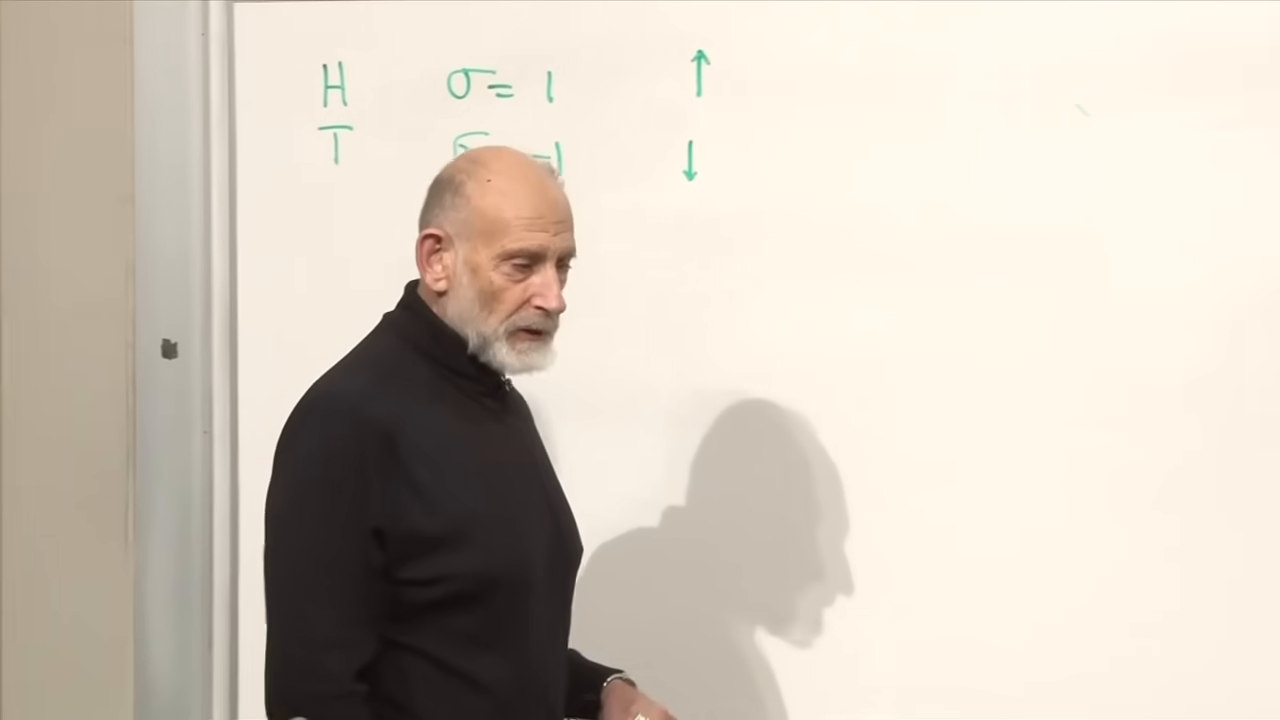
\includegraphics[width=0.78\textwidth]{lecture_01_figure_02.png}
  \caption{黑板上列出等價的標記\(H/T\)、\(\sigma=\pm1\)與上、下箭頭。起初，箭頭只是記號，並不代表經典模型。}
  \lectureframe{00:22:44}
\end{figure}

\begin{classroomqa}
\audiencequestion{正面和反面與這個物理系統有什麼關係？}
\lecturerresponse{除了提供兩個熟悉的名稱之外，沒有其他關係。量子位元在這項測量中有兩種可能結果；正面和反面只是代稱。選用標記\(\pm1\)，是因為它們可以用在方程式中。}
\end{classroomqa}

\subsection{作為黑箱的儀器}

實驗需要第二個系統，也就是儀器\(A\)。目前先把它視為抽象黑箱，具有三項特徵：
\begin{enumerate}
  \item 它有空間取向，以\emph{這一面朝上}標示；
  \item 它有一個能與量子位元互相作用的感測器；
  \item 它有一個起初空白、之後顯示\(+1\)或\(-1\)的顯示器。
\end{enumerate}
探測器的細節刻意留待稍後討論。從操作角度來說，好的探測器由系統與其記錄之間可靠的對應關係來界定。相互作用發生時，觀察者不必正在觀看；儀器可以記錄結果，之後再讀取。

假設顯示器報出\(+1\)。將儀器重設為空白，再立刻重複同一項測量，讓任何獨立演化都還來不及發生。可靠的探測器會再次報出\(+1\)。如果第一次的結果是\(-1\)，立即重複測量也會持續得到\(-1\)：
\begin{equation}
\begin{aligned}
  +1&\longrightarrow +1\longrightarrow +1\longrightarrow\cdots,\\
  -1&\longrightarrow -1\longrightarrow -1\longrightarrow\cdots.
\end{aligned}
\end{equation}
因此，第一次測量可以視為一種\emph{製備}。它使量子位元進入一種態，讓同一項測量在緊接著重複時會得到確定的結果。

可重複性不是可有可無的哲學註解。若沒有它，就沒有操作上的方法可以確認測量結果。有缺陷的儀器可能無法重現結果，但那就不是此處所定義的理想測量。

\begin{classroomqa}
\audiencequestion{這就是波函數坍縮嗎？}
\lecturerresponse{稍後可以引入這種說法。現階段，操作上的描述已經足夠：測量會產生一個結果，並製備出一種態，使同一項測量緊接著再次進行時會重現該結果。替這個過程命名，並不等於解釋了它。}
\end{classroomqa}

\section{取向與經典指針模型的失效}

製備量子位元，使儀器朝上時讀出\(+1\)。將儀器轉過\(180^\circ\)，再重複測量。此時結果是\(-1\)。用倒轉的儀器重複測量，結果仍是\(-1\)；將儀器轉回朝上，結果便恢復為\(+1\)。

這個結果顯示出真正的方向性。上、下記號並非完全任意：反轉探測器會使符號反轉。人們很容易因此認定，量子位元只是小小的向量，而探測器測量的是該向量沿自身軸向的分量。但這個猜想必須經過檢驗，不能逕自相信。

\begin{figure}[htbp]
  \centering
  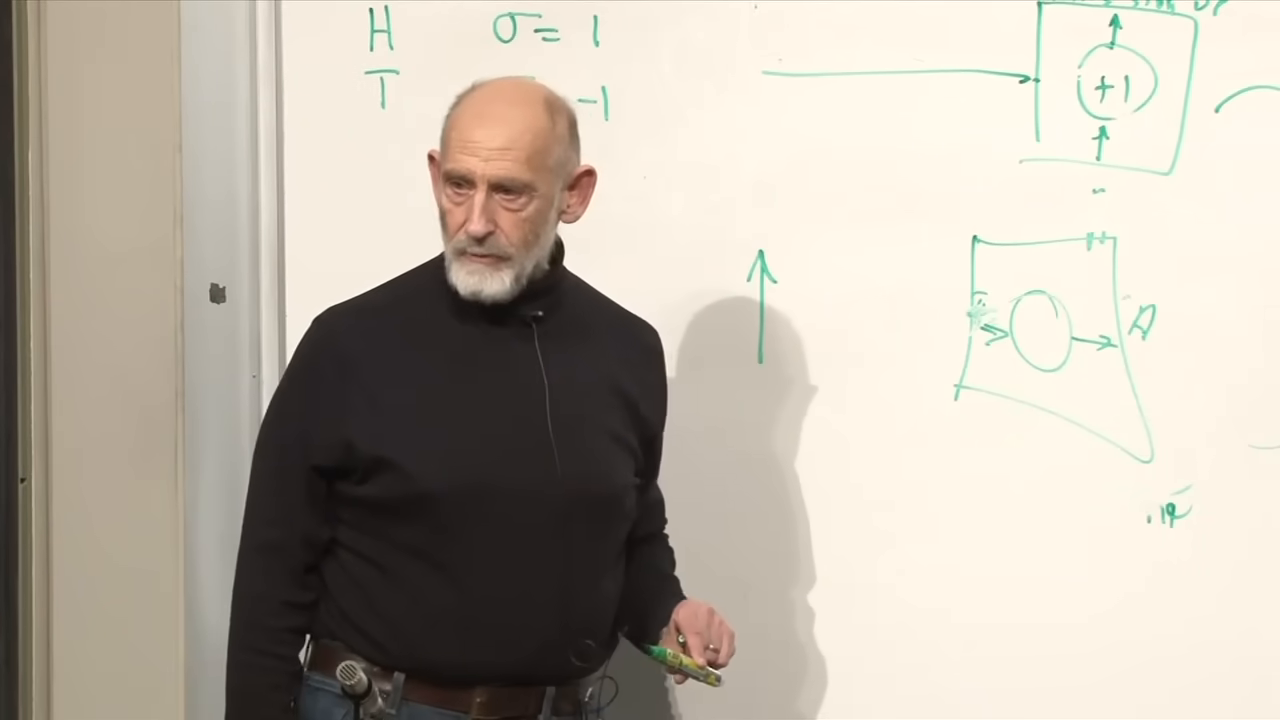
\includegraphics[width=0.82\textwidth]{lecture_01_figure_03.png}
  \caption{黑板上畫著向上製備的量子位元，以及取向各異的分析器。課堂上後來修正了一支粉筆箭頭的方向；這項論證只取決於分析器的軸向。}
  \lectureframe{00:36:21}
\end{figure}

\subsection{側向測量}

將探測器轉過\(90^\circ\)。如果製備好的量子位元是普通的向上指針，它沿水平探測器軸向的分量就會是零：
\begin{equation}
  \hat{\mathbf x}\cdot\hat{\mathbf z}=0.
\end{equation}
量子儀器從不讀出零。每次個別試驗讀出的都是\(+1\)或\(-1\)。

\begin{figure}[htbp]
  \centering
  \resizebox{\linewidth}{!}{%
  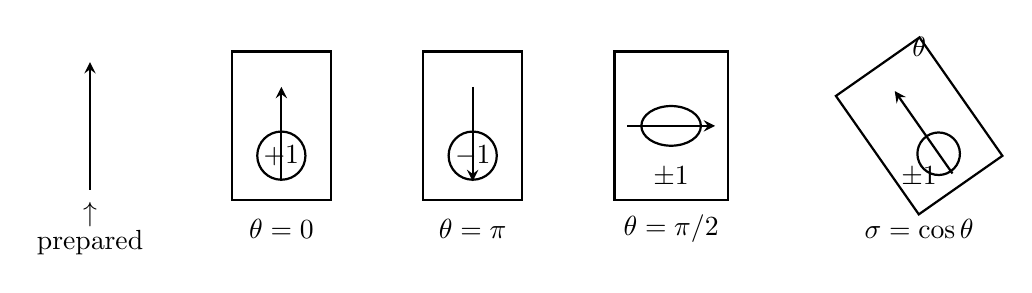
\begin{tikzpicture}[>=stealth,thick,scale=0.90]
    \draw[->] (0,0)--(0,1.8);
    \node at (0,-0.35) {\(\uparrow\)};
    \node at (0,-0.75) {prepared};

    \draw (2.0,-0.15) rectangle (3.4,1.95);
    \draw (2.7,0.48) circle (0.34);
    \draw[->] (2.7,0.12)--(2.7,1.45);
    \node at (2.7,0.48) {\(+1\)};
    \node at (2.7,-0.55) {\(\theta=0\)};

    \draw (4.7,-0.15) rectangle (6.1,1.95);
    \draw (5.4,0.48) circle (0.34);
    \draw[->] (5.4,1.45)--(5.4,0.12);
    \node at (5.4,0.48) {\(-1\)};
    \node at (5.4,-0.55) {\(\theta=\pi\)};

    \draw (7.4,-0.15) rectangle (9.0,1.95);
    \draw (8.2,0.90) ellipse (0.42 and 0.28);
    \draw[->] (7.58,0.90)--(8.82,0.90);
    \node at (8.2,0.18) {\(\pm1\)};
    \node at (8.2,-0.55) {\(\theta=\pi/2\)};

    \begin{scope}[shift={(11.7,0.90)},rotate=35]
      \draw (-0.72,-1.02) rectangle (0.72,1.02);
      \draw (0,-0.48) circle (0.30);
      \draw[->] (0,-0.82)--(0,0.60);
    \end{scope}
    \node at (11.7,0.18) {\(\pm1\)};
    \node at (11.7,-0.55) {\(\expect{\sigma}=\cos\theta\)};
    \node at (11.7,2.02) {\(\theta\)};
  \end{tikzpicture}
  }%
  \caption{分析器序列的重建圖。旋轉會改變統計分布，但不會改變個別試驗可能出現的結果。}
\end{figure}

用朝上的儀器製備大量量子位元，並保留結果為\(+1\)的量子位元。再用側向儀器對每個保留下來的量子位元測量一次。一半試驗得到\(+1\)，另一半得到\(-1\)，系綜平均值為零：
\begin{equation}
  \expect{\sigma}_{\pi/2}=0.
\end{equation}
這個平均值看似經典指針的水平分量為零，但個別測量記錄並非如此。經典值\(0\)在此被兩種離散結果之間的統計平衡取代。

\begin{classroomqa}
\audiencequestion{如果側向測量後不丟棄那個量子位元，而是把它留下來，會怎麼樣？}
\lecturerresponse{假設它第一次側向測量的結果是\(+1\)。對同一個量子位元重複側向測量，會一次又一次得到\(+1\)。第一次側向測量已依照側向軸向製備了它。若要得到一半對一半的統計結果，就必須用許多量子位元重複完整的製備與測量實驗，而不是反覆確認同一個結果。}
\end{classroomqa}

\subsection{不相容的製備}

測量軸向的順序很重要。先沿垂直方向製備\(+1\)，再沿水平方向測量。第一次水平測量的結果是隨機的。一旦得到水平測量結果，緊接著重複同一方向的測量便會得到確定的結果。現在將探測器轉回垂直軸向，垂直測量的結果又變得隨機。

以符號表示，其中\(M_z\)與\(M_x\)分別代表沿兩個軸向的測量：
\begin{equation}
\begin{aligned}
  M_z&:+1,\\
  M_x&:\pm1,\\
  M_x&:\text{same result},\\
  M_z&:\pm1.
\end{aligned}
\end{equation}
中間的\(x\)測量並非只揭露水平分量、同時保留原本的垂直態。它製備了新的態，原先沿垂直方向的確定性也因此消失。

\begin{classroomqa}
\audiencequestion{探測器會記得第一次的答案嗎？它怎麼知道送來的是同一個量子位元，還是新的量子位元？}
\lecturerresponse{可重複性是被測量的量子位元本身的性質，不是探測器暗中比對記憶的結果。測量之後，量子位元處於一種態，使同一項測量緊接著再次進行時會得到相同答案。若送來的是以不同方式製備的量子位元，結果便取決於那項製備。追蹤正在測量哪個物理系統，是一般的實驗室紀錄工作。}
\end{classroomqa}

\begin{classroomqa}
\audiencequestion{所以，觀察的行為會製備那個特定的量子位元嗎？}
\lecturerresponse{是的。測量一旦製備了量子位元，同一項測量就會得到相同答案，直到發生其他演化或介入不相容的測量為止。}
\end{classroomqa}

\section{任意旋轉的分析器}

令探測器軸向與製備系綜時所沿的軸向夾角為\(\theta\)。每次試驗得到的結果仍然是
\begin{equation}
  \sigma=\pm1.
\end{equation}
相對頻率會隨角度改變，使平均值為
\begin{equation}
  \expect{\sigma}_{\theta}=\cos\theta.
  \label{eq:qml1-cosine-mean}
\end{equation}
幾個極限情形是
\begin{align}
  \expect{\sigma}_{0}&=+1,\\
  \expect{\sigma}_{\pi/2}&=0,\\
  \expect{\sigma}_{\pi}&=-1.
\end{align}
在\(\theta=0\)附近，大多數結果是\(+1\)，偶爾出現\(-1\)。在\(\theta=\pi\)附近，大多數結果是\(-1\)，偶爾出現\(+1\)。

\begin{figure}[htbp]
  \centering
  \includegraphics[width=0.82\textwidth]{lecture_01_figure_04.png}
  \caption{任意角度實驗的實際板書：沿垂直方向製備的系綜進入一個傾斜\(\theta\)的分析器。}
  \lectureframe{00:48:55}
\end{figure}

呈現平滑向量式變化的是系綜平均值，而非單次測量結果。若\(p_+(\theta)\)與\(p_-(\theta)\)是兩種結果的機率，則
\begin{equation}
  p_+ + p_-=1,
  \qquad
  p_+-p_-=\cos\theta.
\end{equation}
因此，
\begin{equation}
\begin{aligned}
  p_+(\theta)&=\frac{1+\cos\theta}{2}
  =\cos^2\frac{\theta}{2},\\
  p_-(\theta)&=\frac{1-\cos\theta}{2}
  =\sin^2\frac{\theta}{2}.
\end{aligned}
  \label{eq:qml1-half-angle-probabilities}
\end{equation}
\editorialnote{講課中給出了兩種結果及其平均值\(\cos\theta\)。方程式~\eqref{eq:qml1-half-angle-probabilities}可由這些陳述直接代數推得，並明確寫出其中隱含的頻率定律。}

\begin{classroomqa}
\audiencequestion{未經製備的量子位元集合也會呈現\(\cos\theta\)平均值嗎？}
\lecturerresponse{未極化的集合中沒有選定任何特定方向，因此平均值為零。對\(\theta\)的依賴，是指系綜先沿著一個確定軸向製備的情形。}
\end{classroomqa}

\begin{classroomqa}
\audiencequestion{如果量子位元之間沒有其他動力學演化，為什麼還需要整個系綜？}
\lecturerresponse{對單一量子位元進行第一次傾斜方向的測量，只會得到一個樣本。對同一個量子位元緊接著重複測量，每次都只是在確認該樣本。要進行獨立試驗，就需要以相同方式製備多個量子位元，並各自用傾斜的分析器測量一次。}
\end{classroomqa}

\begin{classroomqa}
\audiencequestion{正號與負號的序列中，是否存在某種規律或高階關聯？}
\lecturerresponse{在這個實驗中，各次試驗假定彼此獨立且不相關。單次試驗的機率取決於\(\theta\)，但這裡並未主張結果序列還有其他排列規律。}
\end{classroomqa}

\subsection{此處做了哪些理想化}

目前先把儀器視為取向可連續調整、讀數卻是離散的經典物體。這種對\emph{系統}與\emph{探測器}的區分只是暫時的。探測器本身也是物理系統，最終必須服從量子力學。完整的描述會將系統與儀器一併處理，但這需要我們尚未掌握的數學工具。

\begin{classroomqa}
\audiencequestion{探測器本身也只是另一個二態系統嗎？}
\lecturerresponse{探測器具有物理態，最終必須納入量子描述。目前我們先採取操作上的區分：量子位元是以量子力學描述的對象，而具有特定取向的探測器則提供穩定的經典記錄。之後必須將這個組合系統視為彼此作用的量子系統來分析。}
\end{classroomqa}

\begin{classroomqa}
\audiencequestion{改變探測器旋轉所繞的軸向，是否會引入比此處單一角度更豐富的結構？}
\lecturerresponse{是的，完整的三維圖像更為豐富。單一平面內的旋轉是其中最簡單的一個面向，並與稍後更完整的處理方式相容。}
\end{classroomqa}

\begin{classroomqa}
\audiencequestion{探測器能否回傳介於\(-1\)與\(+1\)之間的連續值？}
\lecturerresponse{探測器的取向可以連續改變，但理想量子位元的每次讀數仍然是\(+1\)或\(-1\)。取向改變時，機率與平均值會呈現連續變化；個別結果則不會。}
\end{classroomqa}

\section{指針與抽象向量}

現在先把實驗事實與數學分開討論。物理空間中的普通箭頭稱為\emph{指針}。數學向量的概念更一般：它是向量空間中的一個元素，不一定指向普通空間中的任何方向。

\begin{definition}
複向量空間\(V\)是一個向量集合，其中定義了向量加法與複數純量乘法，並滿足通常的線性規則。特別是，對於\(u,v,w\in V\)與\(a,b\in\mathbb C\)，
\begin{align}
  u+v&=v+u,\\
  (u+v)+w&=u+(v+w),\\
  a(u+v)&=au+av,\\
  (a+b)u&=au+bu,\\
  (ab)u&=a(bu),\\
  1u&=u.
\end{align}
空間中有零向量\(0\)；每個\(u\)都有一個加法反元素\(-u\)。
\end{definition}

課堂討論起初只強調運算與封閉性：
\begin{equation}
\begin{aligned}
  u,v\in V&\Longrightarrow u+v\in V,\\
  a\in\mathbb C,\ u\in V&\Longrightarrow au\in V.
\end{aligned}
\end{equation}
之後，課堂上再依提問補充零向量與交換律。其餘熟悉的公理，則明確列出在引入具體的列向量模型時已經用到的性質。

實數構成以\(\mathbb R\)為純量的一維向量空間。複數構成以\(\mathbb C\)為純量的一維向量空間，也構成以\(\mathbb R\)為純量的二維向量空間。複值函數\(\psi(x)\)也構成複向量空間，因為
\begin{equation}
  (\psi+\phi)(x)=\psi(x)+\phi(x),
  \qquad
  (z\psi)(x)=z\psi(x).
\end{equation}
函數空間的例子之後會變得很重要，不過先從有限維列向量入手，較容易看清其中的結構。

\begin{classroomqa}
\audiencequestion{向量與向量空間有什麼不同？}
\lecturerresponse{向量是其中一個元素；向量空間則是所有這類元素的集合，以及對它們進行加法與純量乘法的規則。這就像一個數是單一對象，而數系則是附有運算規則的集合。}
\end{classroomqa}

\section{二分量複數列向量}

用狄拉克記號將抽象向量寫成\(\ket{\alpha}\)。一種具體表示方式是
\begin{equation}
  \ket{\alpha}
  \longleftrightarrow
  \begin{pmatrix}
    \alpha_1\\
    \alpha_2
  \end{pmatrix},
  \qquad
  \alpha_1,\alpha_2\in\mathbb C.
\end{equation}
若
\begin{equation}
  \ket{\beta}
  \longleftrightarrow
  \begin{pmatrix}
    \beta_1\\
    \beta_2
  \end{pmatrix},
\end{equation}
則加法與純量乘法按分量定義：
\begin{align}
  \ket{\alpha}+\ket{\beta}
  &\longleftrightarrow
  \begin{pmatrix}
    \alpha_1+\beta_1\\
    \alpha_2+\beta_2
  \end{pmatrix},\\
  z\ket{\alpha}
  &\longleftrightarrow
  \begin{pmatrix}
    z\alpha_1\\
    z\alpha_2
  \end{pmatrix},
  \qquad z\in\mathbb C.
\end{align}

\begin{figure}[htbp]
  \centering
  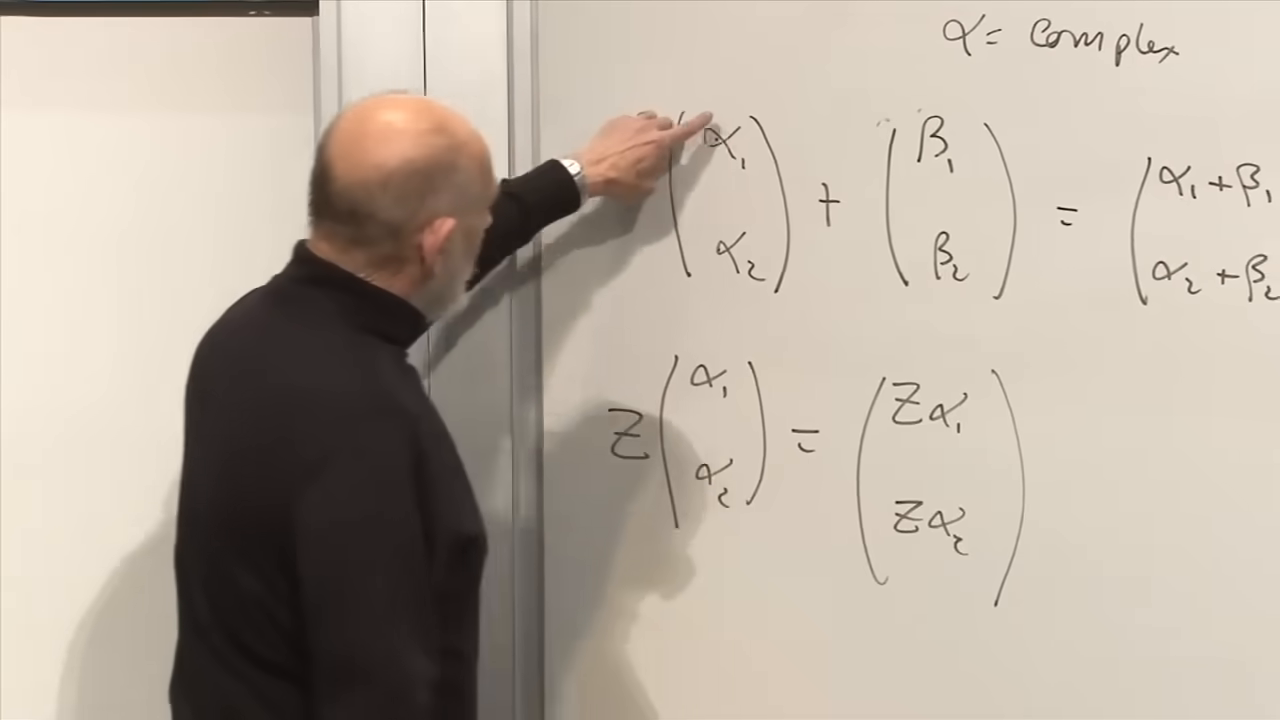
\includegraphics[width=0.88\textwidth]{lecture_01_figure_05.png}
  \caption{兩個複數列向量相加，以及複數純量乘上列向量時的分量運算規則。}
  \lectureframe{01:14:28}
\end{figure}

零向量為
\begin{equation}
  \ket{0}
  =
  \begin{pmatrix}
    0\\
    0
  \end{pmatrix},
  \qquad
  \ket{\alpha}+\ket{0}=\ket{\alpha}.
\end{equation}
三分量列向量構成另一個向量空間，固定為任意其他分量數的列向量亦然。二分量列向量不能與三分量列向量相加，因為兩者屬於不同空間，沒有能將它們的分量逐一對應的加法規則。

\begin{classroomqa}
\audiencequestion{列向量是矩陣嗎？}
\lecturerresponse{一般而言，列向量就是只有一欄的矩陣。在本課程中，「\emph{矩陣}」通常指方形陣列，而只有一欄的陣列稱為列向量。這只是術語上的區分，並不代表代數上有不同看法。}
\end{classroomqa}

\begin{classroomqa}
\audiencequestion{向量相加的順序會有影響嗎？}
\lecturerresponse{不會。逐分量相加沿用了複數加法的交換律：
\[
  \ket{\alpha}+\ket{\beta}
  =
  \ket{\beta}+\ket{\alpha}.
\]
這是向量空間公理之一。}
\end{classroomqa}

\section{對偶向量：左矢與右矢}

每個右矢\(\ket{A}\)在對偶空間中都有一個對應向量，記為\(\bra{A}\)。從右矢到左矢的對應是可加的，但複數純量會取複共軛：
\begin{align}
  \ket{A}+\ket{B}
  &\longleftrightarrow
  \bra{A}+\bra{B},\\
  z\ket{A}
  &\longleftrightarrow
  z^*\bra{A}.
  \label{eq:qml1-antilinear-dual}
\end{align}
第二條規則是複向量空間的關鍵特性。右矢乘上純量後所對應的對偶向量，會乘上該純量的複共軛。

\begin{figure}[htbp]
  \centering
  \includegraphics[width=0.86\textwidth]{lecture_01_figure_06.png}
  \caption{右矢與左矢的對應關係及其兩項規則：向量和會對應到左矢和，純量乘法則要取複共軛。}
  \lectureframe{01:23:15}
\end{figure}

對於二分量的表示方式，
\begin{equation}
  \ket{\alpha}
  =
  \begin{pmatrix}
    \alpha_1\\
    \alpha_2
  \end{pmatrix}
  \qquad\Longrightarrow\qquad
  \bra{\alpha}
  =
  \begin{pmatrix}
    \alpha_1^*&\alpha_2^*
  \end{pmatrix}.
  \label{eq:qml1-bra-from-ket}
\end{equation}
複共軛實現了對偶對應，而行向量記法則清楚區分了這兩類對象。方程式~\eqref{eq:qml1-bra-from-ket}也直接驗證了方程式~\eqref{eq:qml1-antilinear-dual}。

\section{內積}

給定\(\ket{\alpha}\)與\(\ket{\beta}\)，將對應於\(\beta\)的左矢與右矢\(\alpha\)結合：
\begin{equation}
  \braket{\beta}{\alpha}
  =
  \begin{pmatrix}
    \beta_1^*&\beta_2^*
  \end{pmatrix}
  \begin{pmatrix}
    \alpha_1\\
    \alpha_2
  \end{pmatrix}
  =
  \beta_1^*\alpha_1+\beta_2^*\alpha_2.
  \label{eq:qml1-inner-product}
\end{equation}
「\emph{括號}」一詞是由「\emph{左矢}」與「\emph{右矢}」組合而成。這是點積在複數向量中的類比：將對應分量相乘後相加，並在左矢一側取複共軛。

\begin{figure}[htbp]
  \centering
  \includegraphics[width=0.88\textwidth]{lecture_01_figure_07.png}
  \caption{黑板上將內積\(\braket{\beta}{\alpha}\)算為\(\beta_1^*\alpha_1+\beta_2^*\alpha_2\)。}
  \lectureframe{01:31:25}
\end{figure}

交換兩個向量的位置，可得
\begin{equation}
  \braket{\alpha}{\beta}
  =
  \alpha_1^*\beta_1+\alpha_2^*\beta_2
  =
  \braket{\beta}{\alpha}^{*}.
  \label{eq:qml1-conjugate-symmetry}
\end{equation}
因此一般而言，順序會有影響，但兩種順序的結果只差一個複共軛。

\begin{classroomqa}
\audiencequestion{能不能定義一種複向量乘積，而不對其中一側取複共軛？}
\lecturerresponse{可以自行定義這種雙線性表示式，但如此一來，向量與自身的乘積未必是實數或正數。這種結構對量子力學並不實用。取複共軛的厄米內積能提供後續所需的範數與機率結構。}
\end{classroomqa}

\subsection{範數與正定性}

在方程式~\eqref{eq:qml1-inner-product}中令\(\beta=\alpha\)：
\begin{equation}
  \braket{\alpha}{\alpha}
  =
  \alpha_1^*\alpha_1+\alpha_2^*\alpha_2
  =
  |\alpha_1|^2+|\alpha_2|^2.
  \label{eq:qml1-norm-square}
\end{equation}
這個數等於自身的複共軛，因此是實數。它非負，而且只有零向量的內積才為零。長度定義為
\begin{equation}
  \|\alpha\|
  =
  \sqrt{\braket{\alpha}{\alpha}}.
\end{equation}
因此，複數分量仍會給出一般的非負實數長度。

\begin{figure}[htbp]
  \centering
  \includegraphics[width=0.88\textwidth]{lecture_01_figure_08.png}
  \caption{黑板上的自內積：\(\braket{\alpha}{\alpha}=|\alpha_1|^2+|\alpha_2|^2\)，也就是範數的平方。}
  \lectureframe{01:34:40}
\end{figure}

\section{正交性與維度}

兩個向量的內積為零時，稱它們彼此正交：
\begin{equation}
  \braket{\beta}{\alpha}=0.
  \label{eq:qml1-orthogonality}
\end{equation}
由於共軛對稱性，正交關係與向量的順序無關：
\begin{equation}
  \braket{\beta}{\alpha}=0
  \quad\Longrightarrow\quad
  \braket{\alpha}{\beta}
  =
  \braket{\beta}{\alpha}^{*}
  =0.
\end{equation}

在二分量空間中，最簡單的一組正交向量是
\begin{equation}
  \ket{e_1}
  =
  \begin{pmatrix}
    1\\
    0
  \end{pmatrix},
  \qquad
  \ket{e_2}
  =
  \begin{pmatrix}
    0\\
    1
  \end{pmatrix},
  \qquad
  \braket{e_1}{e_2}=0.
  \label{eq:qml1-standard-basis}
\end{equation}

\begin{figure}[htbp]
  \centering
  \includegraphics[width=0.88\textwidth]{lecture_01_figure_09.png}
  \caption{黑板上構造出標準的正交列向量\((1,0)^{\mathsf T}\)與\((0,1)^{\mathsf T}\)。}
  \lectureframe{01:39:50}
\end{figure}

維度可以用一組彼此正交的非零向量所能包含的最大數目來界定。在二維空間中，最多可以有兩個這樣的向量，不可能有第三個。具體而言，令
\begin{equation}
  \ket{v}
  =
  \begin{pmatrix}
    v_1\\
    v_2
  \end{pmatrix}
\end{equation}
它與方程式~\eqref{eq:qml1-standard-basis}中的兩個向量都正交。於是
\begin{equation}
  \braket{e_1}{v}=v_1=0,
  \qquad
  \braket{e_2}{v}=v_2=0,
\end{equation}
因此\(\ket{v}=\ket{0}\)。不存在同時垂直於這兩個向量的第三個非零向量。

\begin{classroomqa}
\audiencequestion{零向量不是與所有向量都正交嗎？那不就多出一個？}
\lecturerresponse{是的，所以定義中必須明確指出是彼此正交的\emph{非零}向量。零向量不代表獨立方向，因此計算維度時不列入。}
\end{classroomqa}

\begin{remark}
在列向量表示法中，維度等於分量數目。正交性的定義則更為抽象，不必先選定座標也能成立。
\end{remark}

\section{黑板上的其他問題}

\begin{classroomqa}
\audiencequestion{函數構成的向量空間也適用相同的結構嗎？}
\lecturerresponse{是的。函數可以視為具有連續指標的一整列分量\(\psi(x)\)。加法與純量乘法都是逐點進行。相應的內積會是積分，而非有限項的總和；稍後會再說明這項建構。}
\end{classroomqa}

\begin{classroomqa}
\audiencequestion{右矢乘上左矢會得到矩陣嗎？}
\lecturerresponse{會。內積\(\bra{\beta}\ket{\alpha}\)將行向量與列向量縮併，得到一個數。若交換順序，\(\ket{\alpha}\bra{\beta}\)則會得到外積，也就是一個方陣。內積與外積之後都會派上用場。}
\end{classroomqa}

\begin{classroomqa}
\audiencequestion{測量真的會影響量子位元，而不只是揭露它原本的狀態嗎？}
\lecturerresponse{會。沿新軸向進行的第一次測量會製備一個新態，因此重複同一方向的測量會確認原結果，轉回舊軸向則會再次出現不確定性。這種不可避免的擾動，正是量子實驗與理想化經典測量的區別；後者原則上可以做到任意微弱。}
\end{classroomqa}

\section{建構的兩個部分}

現在我們有兩個尚未接合的部分。實驗部分告訴我們：
\begin{enumerate}
  \item 理想量子位元測量只有\(\pm1\)這兩種結果；
  \item 緊接著重複同一項測量會確認結果；
  \item 改變探測器軸向會改變測量所製備的態；
  \item 對已製備的系綜而言，分析器傾斜\(\theta\)時，平均值為\(\cos\theta\)。
\end{enumerate}
數學部分則告訴我們：
\begin{enumerate}
  \item 量子態將以向量表示，而非經典點；
  \item 相關向量構成複向量空間；
  \item 右矢有對偶左矢，左矢在複數純量縮放下呈反線性；
  \item 厄米內積定義了長度、正交性與維度。
\end{enumerate}

接下來的任務是把這兩個部分連結起來。量子位元的二維複數狀態空間必須重現分析器實驗中的可重複性、隨機性，以及隨角度變化的統計結果。量子力學正是從這種連結開始，而不是從任何隱藏的古典圖像開始。
